\section{Results}

In this section, we present the results obtained throughout the development of this work, detailing the different approaches and techniques applied for energy consumption prediction.

Initially, we implemented a Random Forest model as our baseline, applying hyperparameter tuning to optimize performance.

Next, we explored three different feedforward neural network (FNN) architectures:
\begin{enumerate}
\item A simple FNN with minimal layers to establish a neural network baseline.
\item A more complex FNN with additional hidden layers and neurons to capture intricate patterns in the energy consumption data.
\item A specialized FNN that trains different variable groups in distinct ways, allowing the model to process different types of features through specialized network paths.
\end{enumerate}

All FNN models were trained for 50 epochs using the processed dataset that included our engineered features, with particular attention to the lag variables that capture temporal dependencies.

Finally, we implemented a Long Short-Term Memory (LSTM) network, a specialized recurrent neural network architecture designed specifically for sequence prediction problems like our time series energy consumption forecasting. This network was trained for 20 epochs using our processed dataset. The LSTM model leverages its ability to remember patterns over long time intervals, making it particularly well-suited for capturing both short-term fluctuations and long-term trends in energy usage. 

Throughout our experiments, model performance was evaluated using standard regression metrics such as Mean Absolute Error (MAE), Root Mean Squared Error (RMSE), and R² score, allowing for comprehensive comparison across the different methodologies.

\subsection{Random Forest}

The first model developed was a Random Forest, intended to serve as a baseline for the prediction task. To ensure robust evaluation, the dataset was split into training, validation, and test sets using a 60\%/20\%/20\% split, respectively. The split was performed randomly while maintaining a representative distribution across all subsets.

The model's initial performance was evaluated on all three sets: training, validation, and test. Without any hyperparameter tuning, the model already demonstrated excellent performance on the training data, as shown in the table below:

\begin{table}[H]
\centering
\caption{Initial Performance of the Random Forest Model}
\begin{tabular}{||c|c|c|c||}
\hline
\textbf{Metric} & \textbf{Training} & \textbf{Validation} & \textbf{Test} \\
\hline
\textbf{MAE} & 0.0276 & 0.0738 & 0.0734 \\
\hline
\textbf{MSE} & 0.0036 & 0.0253 & 0.0248 \\
\hline
\textbf{RMSE} & 0.0597 & 0.1591 & 0.1576 \\
\hline
\textbf{R²} & 0.9987 & 0.9904 & 0.9906 \\
\hline
\end{tabular}
\label{tab:rf_initial_performance}
\end{table}

The model exhibited near-perfect performance on the training set, with an R² score close to 1. However, performance on the validation and test sets showed a slight decline, indicating that while the model generalized well, there was still room for improvement.

\subsubsection{Hyperparameter Tuning}

To enhance performance and prevent potential overfitting, hyperparameter optimization was performed using \textit{RandomizedSearchCV}. The following parameters were considered during the tuning process:

\begin{itemize}
\item \textit{n\_estimators}: Number of trees in the forest.
\item \textit{max\_depth}: Maximum depth of each tree.
\item \textit{min\_samples\_split}: Minimum number of samples required to split an internal node.
\item \textit{min\_samples\_leaf}: Minimum number of samples required to be at a leaf node.
\item \textit{max\_features}: Number of features to consider when looking for the best split.
\end{itemize}

The best combination of hyperparameters obtained through the search is summarized in the table below:

\begin{table}[H]
\centering
\caption{Best Hyperparameters Found}
\begin{tabular}{|c|c|}
\hline
\textbf{Hyperparameter} & \textbf{Value} \\
\hline
\textit{n\_estimators} & 500 \\
\hline
\textit{min\_samples\_split} & 2 \\
\hline
\textit{min\_samples\_leaf} & 2 \\
\hline
\textit{max\_features} & \textit{log2} \\
\hline
\textit{max\_depth} & \textit{None} \\
\hline
\end{tabular}
\label{tab:rf_best_hyperparameters}
\end{table}

After applying the optimal hyperparameters, the model was re-evaluated. While performance on the training set slightly decreased—indicating reduced overfitting—performance on both validation and test sets improved marginally, suggesting better generalization:

\begin{table}[H]
\centering
\caption{Performance After Hyperparameter Tuning}
\begin{tabular}{||c|c|c|c||}
\hline
\textbf{Metric} & \textbf{Training} & \textbf{Validation} & \textbf{Test} \\
\hline
\textbf{MAE} & 0.0391 & 0.0746 & 0.0744 \\
\hline
\textbf{MSE} & 0.0074 & 0.0238 & 0.0237 \\
\hline
\textbf{RMSE} & 0.0859 & 0.1543 & 0.1541 \\
\hline
\textbf{R²} & 0.9972 & 0.9910 & 0.9910 \\
\hline
\end{tabular}
\label{tab:rf_optimized_performance}
\end{table}

Com os novos hiperparâmetros, o modelo manteve um desempenho elevado e consistente nos três conjuntos. Comparado com a versão inicial, observou-se uma leve redução no desempenho sobre os dados de treino (indicando menor sobreajuste), enquanto os resultados nos conjuntos de validação e teste melhoraram ligeiramente. Isso mostra que o modelo ficou mais robusto e generalizou melhor para dados não vistos.


\begin{figure}[H]
\centering
\begin{minipage}{0.48\textwidth}
  \centering
  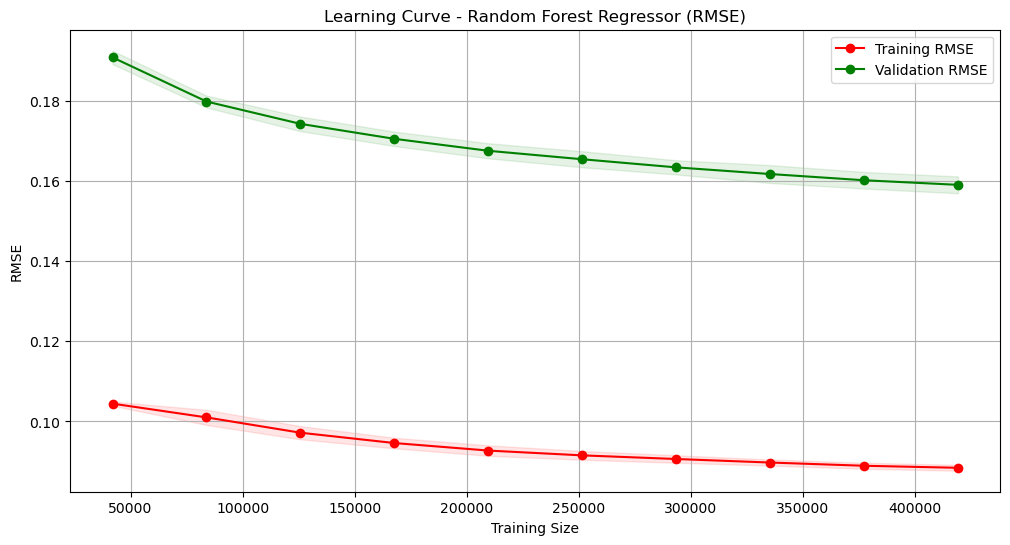
\includegraphics[width=\linewidth]{images/lc-RF-rmse.png}
  \caption{Learning Curve RMSE Random Forest}
  \label{fig:imagem1}
\end{minipage}
\hfill
\begin{minipage}{0.48\textwidth}
  \centering
  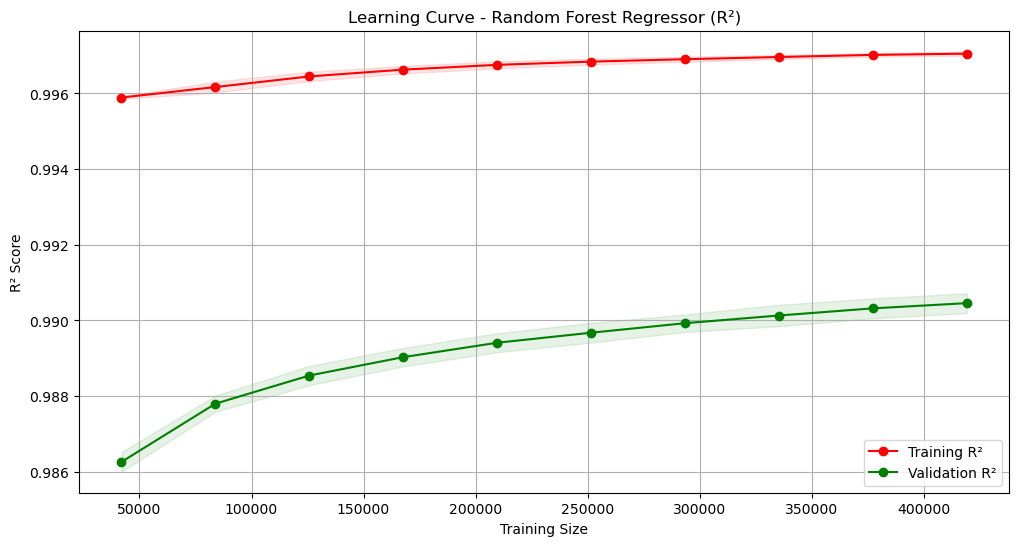
\includegraphics[width=\linewidth]{images/lc-RF-r2.png}
  \caption{Learning Curve $R^2$ Random Forest}
  \label{fig:imagem2}
\end{minipage}
\end{figure}

The learning curves above illustrate the model's behavior during the training process following hyperparameter tuning.

A more detailed analysis of the results shows that the R² score on the training set ranged from 0.994 to 0.998, while on the validation set, it ranged between 0.985 and 0.992. This relatively small difference indicates that the model has strong generalization capabilities, with a low degree of overfitting.

Regarding the RMSE, the values on the training set ranged from 0.12 to 0.07, whereas on the validation set they ranged from 0.19 to 0.15. This discrepancy suggests that the model incurs a slightly higher prediction error on unseen data, although it still maintains robust performance.

Overall, the results demonstrate that the model is well-fitted and generalizes effectively. Nonetheless, there remains some room for improvement in terms of robustness.

\subsection{Feedforward Neural Networks (FNN)}

At this stage, three versions of Feedforward Neural Networks (FNN) were developed, with the objective of comparing different architectures and regularization levels in order to find a balance between performance and generalization. The networks were trained using the Adam optimizer, with the main evaluation metrics being the Mean Absolute Error (MAE), Mean Squared Error (MSE), and the Coefficient of Determination (R²).

The three versions differed in the number of hidden layers, the number of neurons, and regularization techniques such as dropout, and were evaluated on the training, validation, and test sets. The following are the main results obtained for each version.

\subsubsection{FNN 1: Basic Architecture with Dropout Regularization}

The first version of the Feedforward Neural Network (FNN) was designed with a relatively simple architecture, aimed at assessing the performance with moderate regularization using dropout layers. This architecture consists of three dense layers, with 128, 64, and 32 neurons, respectively, and the use of batch normalization to stabilize the training process.

The architecture of the first Feedforward Neural Network (FNN 1) is summarized in the following table:

\begin{table}[h!]
\centering
\caption{Architecture of FNN 1}
\begin{tabular}{|l|c|c|}
\hline
\textbf{Layer\_Type} & \textbf{Output\_Shape} & \textbf{Act\_Function} \\ \hline
Input Layer & (None, input\_dim) & - \\ \hline
Dense Layer (128 neurons) & (None, 128) & ReLU \\ \hline
Batch Normalization & (None, 128) & - \\ \hline
Dropout & (None, 128) & - \\ \hline
Dense Layer (64 neurons) & (None, 64) & ReLU \\ \hline
Batch Normalization & (None, 64) & - \\ \hline
Dropout & (None, 64) & - \\ \hline
Dense Layer (32 neurons) & (None, 32) & ReLU \\ \hline
Dense Output Layer (1 neuron) & (None, 1) & - \\ \hline
\end{tabular}
\label{tab:fnn1_architecture}
\end{table}

The optimizer used is Adam, with a learning rate of 0.001, and the loss function is mean squared error (MSE), appropriate for regression tasks. The metrics monitored during training were MAE, MSE, and R².

\begin{figure}[!h]
    \centering
    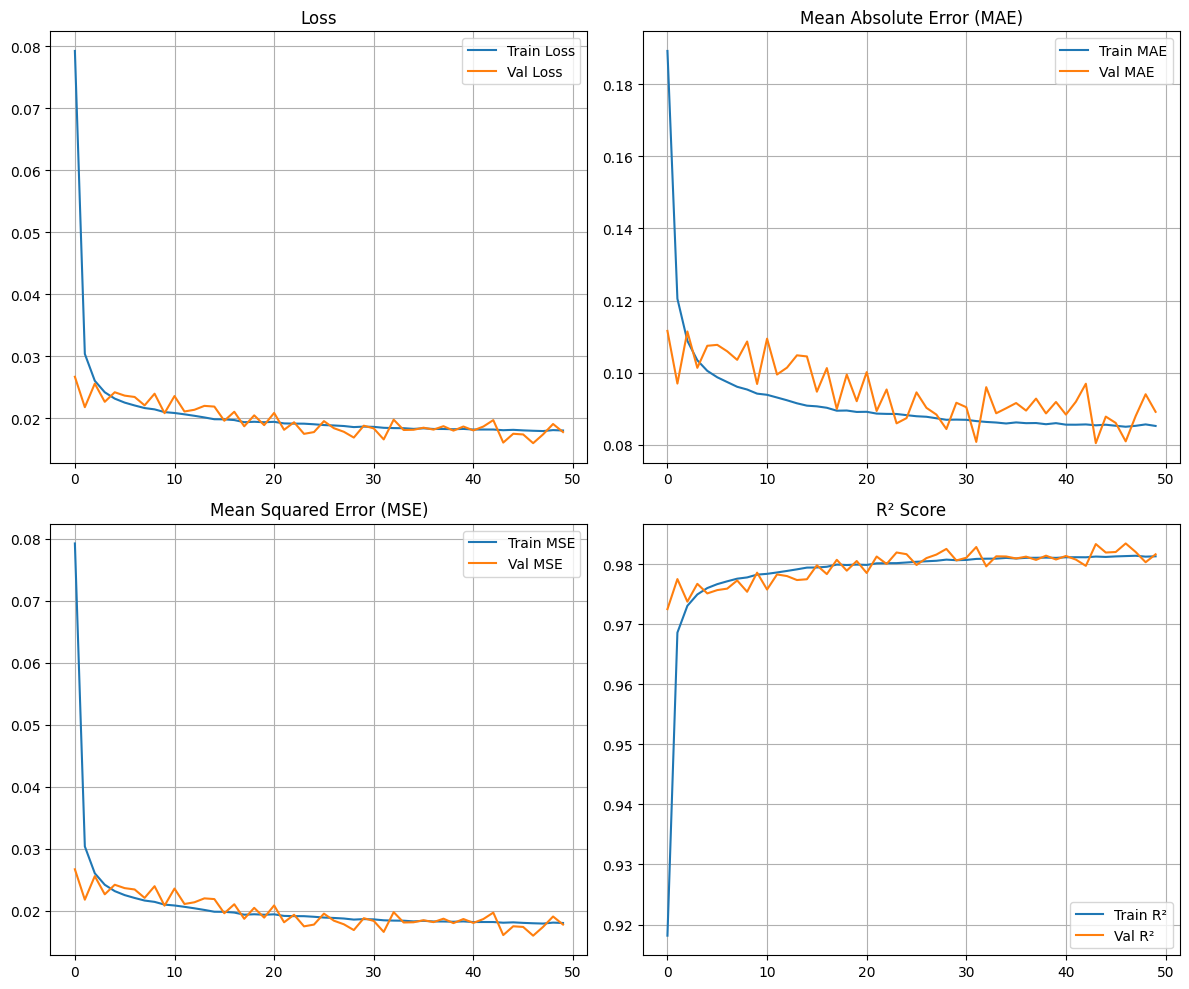
\includegraphics[width=1\linewidth]{images/FNN0-lc.png}
    \caption{FNN 1 learning curves}
    \label{fig:enter-label}
\end{figure}


The learning curves for the first FNN model provide valuable insights into its training behavior and overall performance. The loss curve, shown in the top-left plot, reveals a steep decline in both training and validation loss during the initial epochs. This pattern indicates that the model converged efficiently, learning the underlying patterns in the data without overfitting. The close alignment between training and validation losses further reinforces the model's stability and effectiveness in generalization.

The Mean Absolute Error (MAE) curve, displayed in the top-right, follows a similar trajectory. The error decreases sharply in the early stages and then stabilizes, with training and validation curves closely tracking each other. The absence of significant divergence suggests that the model maintains consistent predictive accuracy across both seen and unseen data, reinforcing its robustness.

Similarly, the Mean Squared Error (MSE), shown in the bottom-left plot, exhibits a rapid decrease followed by stabilization. While the validation MSE presents minor fluctuations, its overall trend remains consistent with the training curve, indicating that the model does not exhibit signs of instability or overfitting.

The R² score curve, presented in the bottom-right, rises quickly during the early epochs and stabilizes above 0.98 after approximately the tenth epoch. The close proximity of the training and validation curves confirms that the model accurately captures the variance in the data and generalizes effectively to new inputs.

In summary, the learning curves collectively indicate that the model is well-tuned and has achieved excellent performance. The consistent behavior across all metrics—loss, MAE, MSE, and R²—demonstrates strong learning capacity and minimal overfitting. 

\begin{table}[H]
\centering
\caption{FNN 1 – Test Set Performance Metrics}
\begin{tabular}{||c|c|c|c|c||}
\hline
\textbf{Metrics} & MAE & MSE & RMSE & R\textsuperscript{2} \\
\hline\hline
\textbf{Values} & 0.1445 & 0.0467 & 0.2161 & 0.9823 \\
\hline
\end{tabular}
\label{tab:fnn1_test_metrics}
\end{table}

The performance on the test set was notably strong, with a Mean Absolute Error (MAE) of 0.1445, Mean Squared Error (MSE) of 0.0467, Root Mean Squared Error (RMSE) of 0.2161, and a Coefficient of Determination (R²) of 0.9823. These results indicate that the model can explain approximately 98.23\% of the variance in the target variable, which is a clear indication of high predictive capability.

The relatively low RMSE suggests that the model's prediction errors are well within acceptable bounds, particularly given the complexity of the data. Combined with the consistent and stable learning curves, these outcomes affirm that the model is both effective and well-generalized. Nonetheless, while FNN 1 achieves robust performance, there remains room for refinement. After this, we explore deeper architectures and alternative regularization strategies to further reduce prediction error and enhance overall robustness.

\begin{figure}[H]
    \centering
    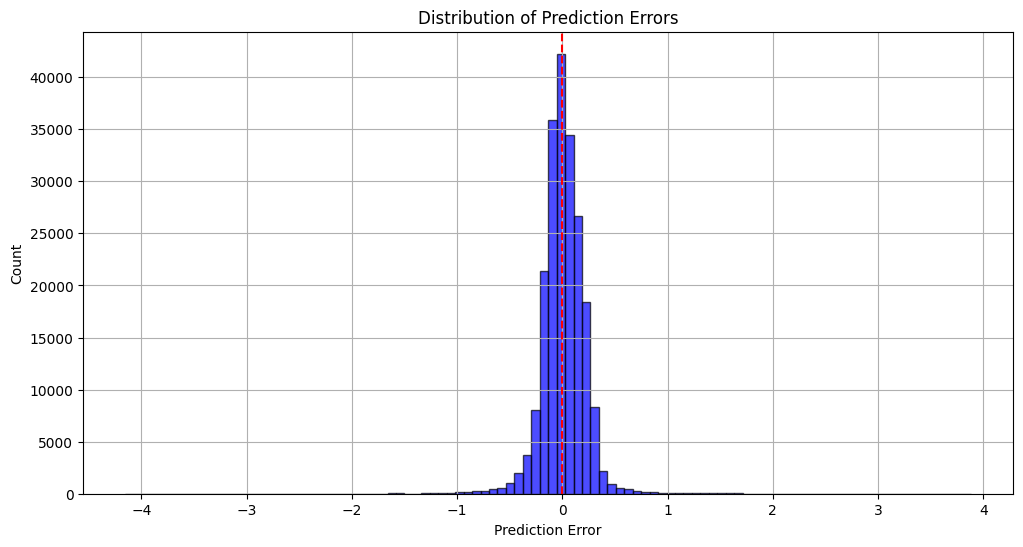
\includegraphics[width=0.8\linewidth]{images/fnn0-de.png}
    \caption{Distribution of Prediction Errors}
    \label{fig:enter-label}
\end{figure}

The histogram of the prediction errors (calculated as actual values minus predicted values) shows a distribution that is centered very close to zero, with the red vertical line likely representing the mean error (0.0090), positioned just slightly above zero. This suggests that the model has minimal bias, as the errors are nearly symmetrically distributed around zero.

The shape of the distribution is approximately normal, which is ideal for a regression model. A normal distribution of errors implies that the model's errors are random, with no obvious patterns, rather than systematic. This indicates that the model is generalizing well and not making consistent mistakes in any specific direction.

The spread of the errors is relatively tight, concentrated between approximately -1 and +1, with very few errors exceeding this range. This suggests that the model's predictions are highly accurate, with most of the predictions being very close to the actual values.

\subsubsection{FNN 2: Deep Architecture with Strong Regularization}

The second Feedforward Neural Network (FNN 2) was designed with a deeper architecture and stronger regularization, aiming to evaluate whether a more complex model could yield better generalization and predictive performance. This version significantly increases the number of layers and neurons, incorporating dropout after each dense layer to mitigate overfitting.

The architecture of FNN 2 is detailed in Table~\ref{tab:fnn2_architecture}.

\begin{table}[h!]
\centering
\caption{Architecture of FNN 2}
\begin{tabular}{|l|c|c|}
\hline
\textbf{Layer\_Type} & \textbf{Output\_Shape} & \textbf{Act\_Function} \\ \hline
Input Layer & (None, input\_dim) & - \\ \hline
Dense Layer (512 neurons) & (None, 512) & ReLU \\ \hline
Batch Normalization & (None, 512) & - \\ \hline
Dropout (0.3) & (None, 512) & - \\ \hline
Dense Layer (256 neurons) & (None, 256) & ReLU \\ \hline
Batch Normalization & (None, 256) & - \\ \hline
Dropout (0.3) & (None, 256) & - \\ \hline
Dense Layer (128 neurons) & (None, 128) & ReLU \\ \hline
Batch Normalization & (None, 128) & - \\ \hline
Dropout (0.3) & (None, 128) & - \\ \hline
Dense Layer (64 neurons) & (None, 64) & ReLU \\ \hline
Batch Normalization & (None, 64) & - \\ \hline
Dropout (0.3) & (None, 64) & - \\ \hline
Dense Layer (32 neurons) & (None, 32) & ReLU \\ \hline
Batch Normalization & (None, 32) & - \\ \hline
Dropout (0.3) & (None, 32) & - \\ \hline
Dense Output Layer (1 neuron) & (None, 1) & - \\ \hline
\end{tabular}
\label{tab:fnn2_architecture}
\end{table}

This model uses the Adam optimizer with a learning rate of 0.001 and is trained to minimize the mean squared error (MSE). The performance metrics monitored throughout training include MAE, MSE, and R².

\begin{figure}[H]
    \centering
    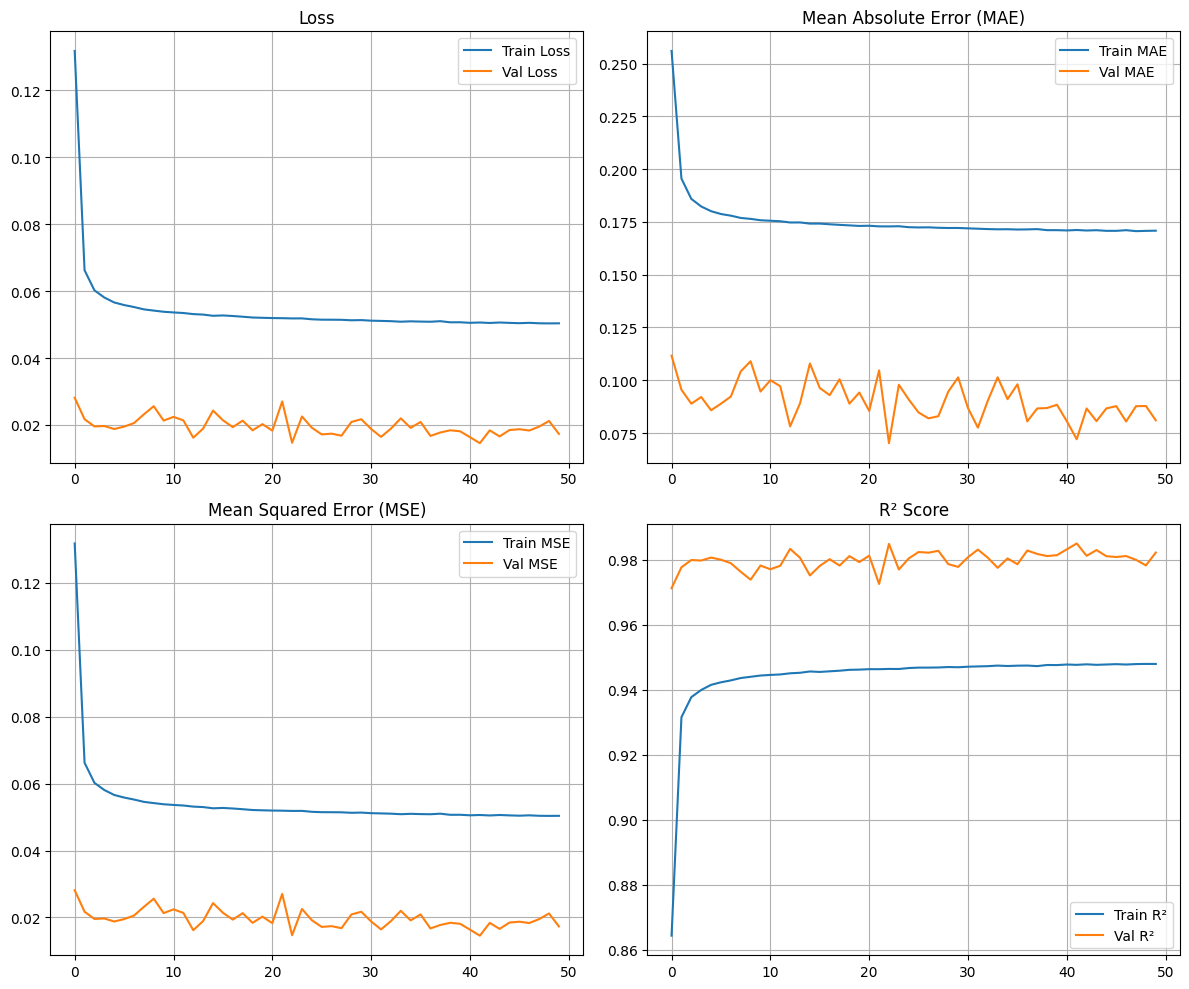
\includegraphics[width=1\linewidth]{images/fnn1-lc.png}
    \caption{FNN 2 learning curves}
    \label{fig:fnn2_learning_curves}
\end{figure}

The learning curves for FNN 2 (Figure~\ref{fig:fnn2_learning_curves}) provide insightful details into the model’s training behavior and its generalization capability. The loss curve (top-left) indicates that the training loss decreases sharply within the first 10 epochs and then stabilizes around 0.05. Notably, the validation loss is consistently lower—hovering around 0.02 throughout training—which is an atypical but encouraging sign that the model generalizes well to unseen data. This consistent gap, where validation outperforms training, suggests an unusual scenario, potentially explained by factors such as data distribution differences or the impact of regularization during training.

The MAE curve (top-right) mirrors the behavior of the loss function. The training MAE decreases and stabilizes at approximately 0.17, whereas the validation MAE remains lower at around 0.09, with minimal fluctuations. The persistent difference indicates that the model is less precise on the training data than on the validation set, a rare occurrence in deep learning. However, the low and stable validation MAE confirms excellent predictive capability on unseen data.

Similarly, the MSE curve (bottom-left) shows that training MSE declines steadily and stabalize near 0.05, while validation MSE holds consistently near 0.02. These results are in line with the loss and MAE plots, reinforcing the conclusion that the model has developed stable predictive power and is not overfitting.

The R² score plot (bottom-right) demonstrates that the training R² begins around 0.86 and gradually increases to stabilize at approximately 0.95. Interestingly, the validation R² starts higher, near 0.975 and remains consistently above the training score throughout the training process. This further supports the notion that the validation set may be easier to predict or exhibits slightly different characteristics than the training data.

In summary, the learning curves of FNN 2 suggest that the model is highly stable, well-regularized, and effective in generalization. All monitored metrics converge after about 10 epochs, implying that additional training is unlikely to yield substantial performance gains. The consistently superior validation performance is atypical and may be attributed to differences in data complexity, sampling strategies, or the effect of dropout and batch normalization disproportionately influencing training dynamics. Nonetheless, the observed behavior indicates that the model is performing reliably across data splits and achieving a high level of accuracy and generalization.

\begin{table}[h!]
\centering
\caption{FNN 2 – Test Set Performance Metrics}
\begin{tabular}{||c|c|c|c|c||}
\hline
\textbf{Metrics} & MAE & MSE & RMSE & R\textsuperscript{2} \\
\hline \hline
\textbf{Values} & 0.1312 & 0.0452 & 0.2125 & 0.9829 \\
\hline
\end{tabular}
\label{tab:fnn2_test_metrics}
\end{table}

The test performance further corroborates the effectiveness of FNN 2. With a Mean Absolute Error of 0.1312, MSE of 0.0452, RMSE of 0.2125, and an R² score of 0.9829, the model clearly demonstrates a high degree of accuracy and a strong ability to explain variance in the target variable. These metrics reflect a slight improvement over FNN 1 and validate the decision to expand the model depth and apply stronger regularization techniques.

\begin{figure}[!h]
    \centering
    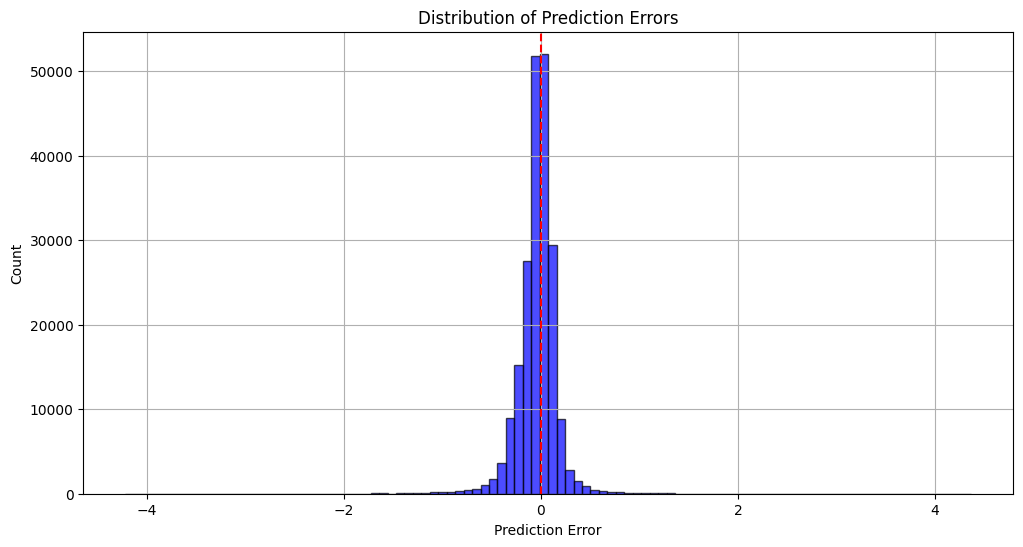
\includegraphics[width=0.8\linewidth]{images/fnn1-de.png}
    \caption{Distribution of Prediction Errors}
    \label{fig:enter-label}
\end{figure}


The errors are centered very near zero, with the red vertical line marking the mean error at approximately \−0.0388. This slight negative shift suggests a minimal and negligible bias in the model's predictions, indicating that, on average, the model slightly overestimates the target values. However, the small magnitude of this bias confirms that the model remains well calibrated overall.

The distribution follows a roughly normal shape, indicating that the model's errors are randomly distributed rather than being systematic. Such a pattern is desirable in regression tasks, as it suggests the absence of structural weaknesses or biases in the model's predictions.

The spread of the errors is narrow, with the majority of predictions falling within a range of approximately \−1 to +1. The standard deviation of the prediction error is 0.2089, reinforcing the model’s consistent accuracy across diverse input conditions. The low variance highlights that most predictions deviate only slightly from the actual values.

\subsubsection{Final Considerations on Tested Architectures}

In addition to the FNN 1 and FNN 2 models detailed earlier, several other experiments were conducted with alternative architectures, including networks with greater depth, different combinations of layers (with and without \textit{Batch Normalization}), and the use of additional regularization techniques like \textit{L2} and \textit{Dropout} in various configurations. However, none of these approaches resulted in significant improvements in the key performance indicators when compared to the two models presented, which proved superior in terms of stability and predictive capability.

Seeking to explore a different approach, a \textit{multi-input model} was also developed, in which the features were logically grouped into sets related to the building, weather variables, temporal lags, and primary use of the building. While this model is simpler in its internal structure, it demonstrated competitive performance on the test set, with \textbf{MAE of 0.1251}, \textbf{MSE of 0.0430}, \textbf{RMSE of 0.2073}, and \textbf{R\textsuperscript{2} of 0.9837}, slightly outperforming the previous models.

Distribution of prediction errors analysis for this model revealed a \textbf{mean error of just 0.0033} and a \textbf{standard deviation of 0.2073}, suggesting not only low bias but also high consistency in predictions. However, due to the grouping of variables into distinct blocks, the learning curves obtained did not provide enough visibility or granularity to allow for a full evaluation of the model’s behavior during training. Despite this visual limitation, the quantitative results demonstrate that the multi-input architecture represents a promising alternative, with potential to be further explored in future work.


\subsection{Long Short-Term Memory (LSTM)}
The last model developed was a simple LSTM network that contained a single LSTM layer which processes the whole temporal sequence. The intuition behind such a simple architecture (of only one layer) is to make comparisons among the previously developed models. An initial training was performed using the default hyperparameters of keras LSTM layer. This model presented great performance metrics when tested.

Right after our first training, we hyper-tuned our model using a grid search approach where the number of units and the recurrent dropout were changed:
\begin{itemize}
    \item num\_units or "hidden size" is analogous to the number of "neurons" in a given layer of a neural network. An LSTM layer contains one or many LSTM cells - the quantity of cells depends on the number of temporal steps. Each of those cells contains a number of units which is defined by the hyperparameter num\_units \cite{ref_num_units}.
    \item The recurrent\_dropout is the fraction of the units to drop for the linear transformation of the recurrent state.
\end{itemize}

The number of units assumed the following values: {32, 64, 128}, and the recurrent dropout assumed the value 0, meaning the recurrent dropout was disabled, and 0.2. After the training phase, the models were tested and the results of the LSTM architecture using the trained hyperparameters is present in the following table.

\begin{table}[H]
\centering
\caption{LSTM model results}
\begin{tabular}{||c|c|c|c|c|c||}
\hline
\textbf{Units} & \textbf{Rec. Dropout} & \textbf{MAE} & \textbf{MSE} & \textbf{RMSE} & \textbf{R²}\\
\hline
32 & 0.0 & 0.111 & 0.041 & 0.203 & 0.984 \\
\hline
32 & 0.2 & 0.105 & 0.039 & 0.198 & 0.985 \\
\hline
64 & 0.0 & 0.104 & 0.037 & 0.191 & 0.986 \\
\hline
64 & 0.2 & 0.098 & 0.034 & 0.184 & 0.987 \\
\hline
128 & 0.0 & 0.096 & 0.032 & 0.179 & 0.988 \\
\hline
128 & 0.2 & 0.093 & 0.032 & 0.180 & 0.988 \\
\hline
\end{tabular}
\label{tab:lstm_performance}
\end{table}

In the table we can see that even though the hyperparameters varied in a quite large range, the test results of our models were very close to each other. Now, taking into consideration the model with the best \(R^2\) let us examine the loss and \(R^2\) performance metric over epochs for both training and validation.

\begin{figure}[H]
    \centering
    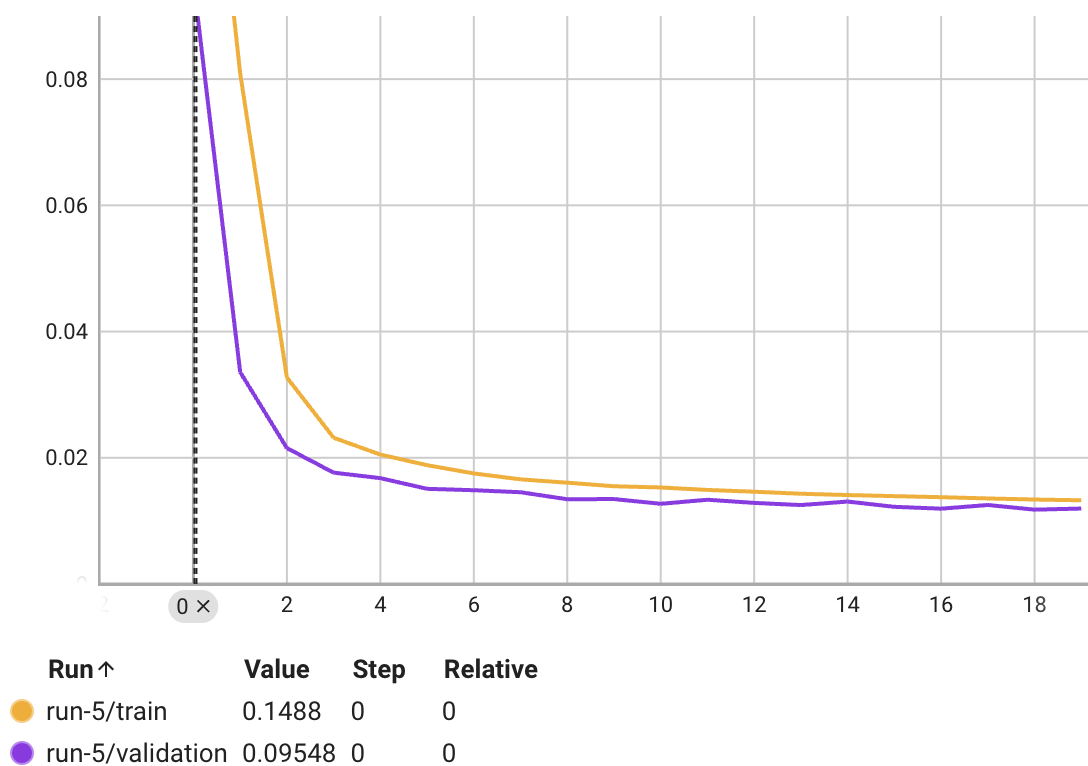
\includegraphics[width=0.75\linewidth]{images/lstm_loss_epoch.png}
    \caption{Loss per epoch}
    \label{fig:lstm_loss_epoch}
\end{figure}
\begin{figure}[H]
    \centering
    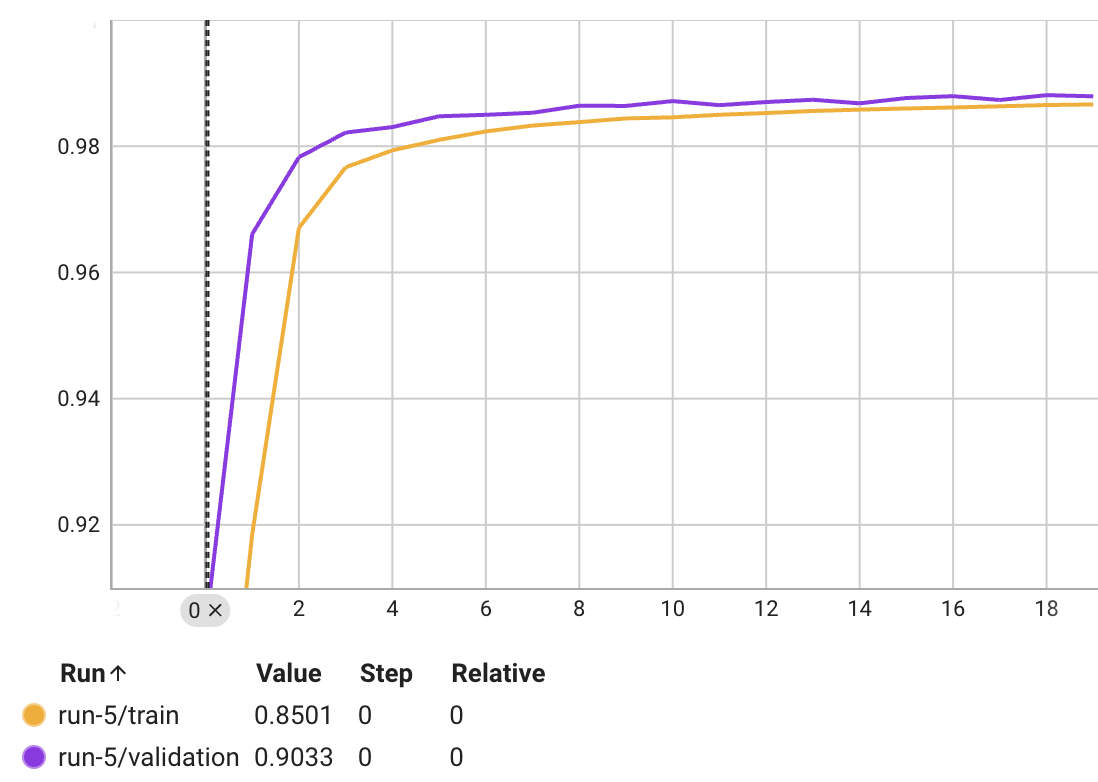
\includegraphics[width=0.75\linewidth]{images/lstm_r2_epoch.png}
    \caption{\(R^2\) per epoch}
    \label{fig:lstm_r2_epoch}
\end{figure}

As seen in the images above, both the loss and \(R^2\) have quickly converged around the fourth epoch. The remaining of the training process seems not to have impact on the performance of our LSTM model. The behaviour of both the validation and training curves suggests optimal learning of the model without signs of overfitting/underfitting.
